\documentclass{article}

\title{Shah Rrks's Dotted Paper}

\usepackage{geometry}


\geometry{a4paper, margin=2mm, top = 20mm}

\usepackage{tikz}
\tikzset{x=1mm, y=1mm}


\newcommand{\sub}{Mathe 2} % Subject's Name 
\newcommand{\aut}{Shah Rrks}
\newcommand{\cha}{Lineare Algebra}
%\pagenumbering{gobble}

\definecolor{DotsColor}{HTML}{000000}
\definecolor{BordersColor}{HTML}{000000}
\definecolor{PageNumbersColor}{HTML}{000000}

%\pagestyle{empty}


%%%%%% Document Begins %%%%%%%%
\begin{document}





\newsavebox{\firstLine}
\savebox{\firstLine}
{
	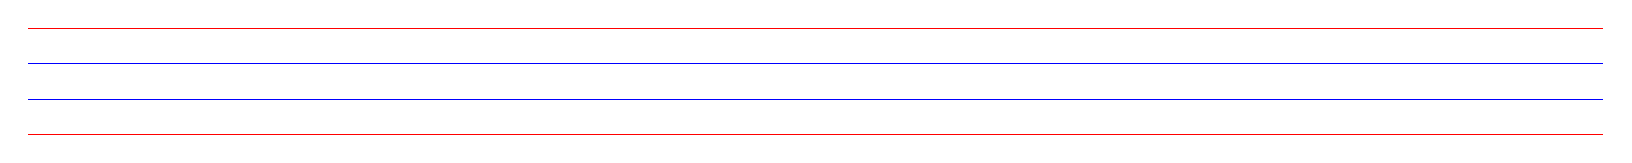
\begin{tikzpicture}

        \draw[color=red] (0,0) -- (200,0);
        \draw[color=blue,thin] (0,4.5) -- (200,4.5); 
        \draw[color=blue,thin] (0,9) -- (200,9); 
        \draw[color=red] (0,13.5) -- (200,13.5); 
     \end{tikzpicture}
}


\newsavebox{\frontPage}
\savebox{\frontPage}
{
\foreach \s in {0,...,12}
{
	\usebox{\firstLine}
    \vspace*{6mm}
}
}


\foreach \m in {0,...,12}
{
	\usebox{\frontPage}


    \newpage 
}






\end{document}